\chapter{Análisis climático y estadístico}
\label{ch:clima_estadistica}

\section{Papel del bloque dentro de HYDRA}

El bloque climático-estadístico constituye el núcleo metodológico de \hydra. Transforma datos históricos y proyecciones climáticas en información directamente útil para simulación, selección de eventos, evaluación probabilística y generación de escenarios. Esta capa actúa como puente entre los datos adquiridos por el bloque de fuentes y los modelos físicos del bloque de modelización.

El bloque se divide en cinco submódulos: \texttt{climate.time\_series} para análisis de extremos y detección de eventos, \texttt{climate.spatial\_analysis} para dependencia espacial y análisis regional, \texttt{climate.stochastic\_generation} para generación sintética de precipitación y caudal, \texttt{climate.bias\_correction} para ajuste de modelos climáticos, y \texttt{climate.hybrid\_downscaling} para reconstrucción masiva de impactos hidráulicos. En conjunto, estos cinco submódulos dan soporte a las cuatro primeras tareas del plan de investigación.

La función de este capítulo es separar tres niveles que a menudo se mezclan en aplicaciones prácticas. El primero es estadístico: estimar distribuciones, dependencias e incertidumbre a partir de series limitadas. El segundo es generativo: producir eventos o series sintéticas que amplían el espacio de escenarios plausibles. El tercero es operacional: reducir el número de simulaciones físicas sin perder cobertura del espacio de impactos. \pyhydra organiza estos niveles en submódulos separados para que cada decisión sea auditable: qué datos entran, qué hipótesis se ajustan, qué escenarios se generan y qué parte se simula explícitamente.

Las salidas del bloque no son resultados finales por sí mismas. Un cuantil de precipitación, una muestra de cópula o una serie CMIP6 corregida solo adquieren significado dentro de una cadena completa que incluye modelización hidrológica/hidráulica y métricas de impacto. Esta es la razón por la que el capítulo insiste en la trazabilidad de parámetros, semillas, tasas de ocurrencia y metadatos de origen.

\section{Análisis temporal y extremos}

\subsection{Detección de eventos}

El módulo \texttt{time\_series.events} implementa dos estrategias complementarias para identificar eventos hidrológicos extremos en series temporales:

\begin{description}
  \item[\texttt{extract\_block\_maxima}] Extrae el máximo de cada bloque temporal definido por una frecuencia (\texttt{YE} para máximos anuales, \texttt{ME} para mensuales). Produce la muestra para el análisis GEV clásico.

  \item[\texttt{extract\_pot}] Extrae picos independientes sobre un umbral con separación mínima entre eventos configurable. La separación mínima es el parámetro crítico para garantizar la independencia de los eventos, y debe ajustarse al tiempo de concentración de la cuenca o al tiempo de decaimiento de la variable analizada.

  \item[\texttt{extract\_discharge\_events}] Detecta eventos de crecida completos por cruce de umbral, con refinamiento en los puntos de inflexión del hidrograma, y extrae para cada uno el valor pico, la duración y el volumen. Esta función es el punto de entrada para el análisis multivariante mediante cópulas. El módulo ofrece variantes equivalentes para precipitación (\texttt{extract\_precipitation\_events}, por rachas húmedas; \texttt{extract\_precipitation\_events\_pot}, por picos sobre umbral; \texttt{extract\_precipitation\_events\_nday}, por acumulación en ventana de $N$ días) y una función unificada de entrada, \texttt{extract\_events}, que selecciona el método según el tipo de variable.
\end{description}

La detección de eventos es una decisión metodológica, no una operación neutra. La duración mínima entre picos, el umbral POT o la definición de volumen condicionan la muestra que después se ajusta con GEV/GPD o se utiliza en una cópula. Por eso las funciones devuelven no solo valores máximos, sino también fechas, duración, volumen y metadatos de extracción. En estudios de impacto, conservar el evento completo es esencial porque el mismo caudal punta puede producir impactos distintos si cambia la duración o la forma del hidrograma.

\subsection{Ajuste de distribuciones de extremos}

El módulo \texttt{time\_series.extremes} implementa el ajuste de distribuciones GEV (Generalized Extreme Value) y GPD (Generalized Pareto Distribution) \parencite{coles2001extremes} con tres métodos:

\begin{description}
  \item[Máxima verosimilitud (MLE)] Estimación clásica por máxima verosimilitud con ajuste de los tres parámetros GEV ($\mu$, $\sigma$, $\xi$). Se calcula mediante \texttt{scipy.stats.genextreme}. Es el método más rápido pero sensible a muestras pequeñas.

  \item[L-momentos] Estimación por L-momentos de primer a cuarto orden \parencite{hosking1997rfa}. Los L-momentos son más robustos que los momentos clásicos ante la presencia de valores extremos, lo que los hace recomendables cuando la muestra es inferior a 30 años. Se usa como método por defecto cuando no se especifica ningún otro.

  \item[Inferencia bayesiana por MCMC] La función \texttt{fit\_gev\_mcmc} ajusta el modelo GEV mediante muestreo MCMC con PyMC \parencite{salvatier2016pymc} y el muestreador NUTS, con una parametrización no centrada. La configuración por defecto usa 4 cadenas con 2000 muestras, lo que produce estimaciones de la distribución posterior de los tres parámetros y, por tanto, intervalos de credibilidad completos para cualquier nivel de retorno. Este método es el más costoso computacionalmente, pero produce las estimaciones más informativas sobre incertidumbre. Para el análisis regional jerárquico (véase más adelante en este capítulo), la clase \texttt{HierarchicalGEV} ofrece además un respaldo alternativo con PyStan \parencite{carpenter2017stan} cuando PyMC no está disponible.

  \item[Aproximación de Fisher] La función \texttt{fit\_gev\_fisher} estima la incertidumbre paramétrica mediante la matriz de información de Fisher, produciendo muestras de la distribución asintóticamente gaussiana de los parámetros sin recurrir a MCMC. Es un intermedio entre MLE y la inferencia bayesiana completa.
\end{description}

La \cref{fig:gev_comparacion} muestra una salida real del notebook general \path{climate/extreme_value_analysis.ipynb}: una comparación entre niveles de retorno estimados con GEV sobre máximos anuales y GPD sobre excedencias POT. La figura permite comprobar visualmente si ambas formulaciones son coherentes en el rango observado y cómo divergen al extrapolar hacia períodos de retorno altos.

La comparación sistemática sobre datos reales se realiza en el caso de la precipitación extrema del 29 de octubre de 2024 en la Comunidad Valenciana (\cref{sec:caso_valencia}), que permite contrastar MLE, L-momentos y MCMC sobre las mismas series observadas, con y sin incluir el evento extraordinario, y documentar el cambio en los niveles de retorno y la incertidumbre de cada método \parencite{navas2025valenciaIA}.

\begin{figure}[htbp]
  \centering
  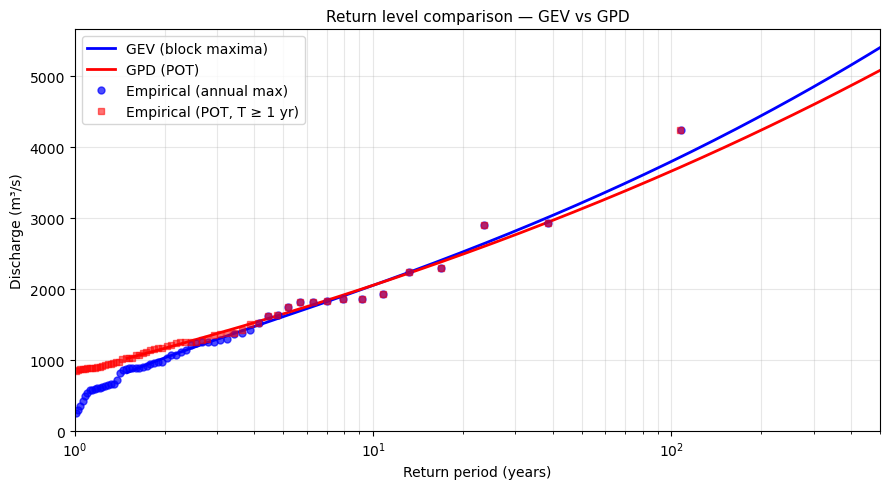
\includegraphics[width=0.88\linewidth]{figures/fig_gev_comparacion_notebook.png}
  \caption{Comparación de niveles de retorno obtenida en el notebook \texttt{climate/extreme\_value\_analysis.ipynb}. La curva azul corresponde al ajuste GEV sobre máximos anuales; la roja, al ajuste GPD sobre excedencias POT. Los puntos muestran posiciones empíricas de máximos anuales y excedencias POT con período de retorno anual o superior. Salida computada del notebook de análisis de extremos de \pyhydra.}
  \label{fig:gev_comparacion}
\end{figure}

Esta comparación no selecciona automáticamente un modelo; sirve como diagnóstico de coherencia entre enfoques de bloques máximos y umbrales. La elección final depende del tamaño muestral, la independencia de las excedencias, la estabilidad del umbral y el comportamiento de cola. Esta distinción es relevante para el diseño de \hydra: el módulo ofrece varios estimadores para facilitar el diagnóstico y la comparación, no para seleccionar uno de ellos sin evaluar los datos y los supuestos del caso.

La función \texttt{return\_levels} calcula los cuantiles para una lista de períodos de retorno a partir de los parámetros ajustados, con intervalos de confianza calculados por bootstrap o por la distribución posterior según el método empleado.

El diseño del módulo evita presentar un único estimador como solución universal. MLE es útil para diagnóstico rápido y muestras largas; L-momentos suele ser más estable en muestras cortas; MCMC permite comunicar incertidumbre paramétrica de forma explícita, pero exige revisar convergencia y sensibilidad a priors. La comparación entre métodos, más que la elección automática de uno, es el valor operativo de \pyhydra en episodios extremos como Valencia 2024.

\section{Análisis espacial}

\subsection{Análisis de frecuencia regional}

El módulo \texttt{spatial\_analysis.rfa} implementa el análisis de frecuencia regional (AFR) mediante el método del índice de avenida (\emph{index-flood}) \parencite{hosking1997rfa} basado en L-momentos. El procedimiento sigue las etapas estándar:
\begin{enumerate}
  \item Ajuste de GEV en cada estación, por máxima verosimilitud (\texttt{fit\_gev\_mle}), L-momentos (\texttt{fit\_gev\_lmom}, requiere \texttt{lmoments3}) o inferencia bayesiana (\texttt{fit\_gev\_bayes}).
  \item Diagnóstico regional mediante el estadístico de discordancia de Hosking--Wallis (\texttt{regional\_discordancy}) y el estadístico de heterogeneidad $H_1$ (\texttt{regional\_heterogeneity}), cuando el número y longitud de las estaciones permiten interpretarlos.
  \item Normalización de cada serie por su índice de avenida —la media de sus máximos anuales— mediante \texttt{regional\_index\_flood}.
  \item Ajuste de la distribución regional sobre los datos normalizados agrupados (\texttt{fit\_regional\_gev}).
  \item Reconversión a cuantiles locales por estación mediante el índice de avenida (\texttt{regional\_return\_levels}).
\end{enumerate}

La función \texttt{fit\_regional\_gev} acepta un diccionario de series de estación y devuelve los parámetros regionales junto con la serie de índices de avenida; \texttt{regional\_return\_levels} aplica el reescalado a cada estación para una lista de períodos de retorno. Además de los ajustes MLE y por L-momentos, la API admite \texttt{method=\textquotesingle{}bayes\textquotesingle{}}, que devuelve medianas e intervalos creíbles de cuantiles regionales escalados por estación. Los diagnósticos de discordancia y heterogeneidad ayudan a detectar estaciones incompatibles o regiones no homogéneas, pero no sustituyen el criterio hidrológico: la delimitación regional debe justificarse por coherencia climática, topográfica y pluviométrica antes de interpretar el ajuste. Su aplicación al caso Valencia 2024 \parencite{navas2025valenciaIA} con tres escalas espaciales (individual, regional local con 9 estaciones, regional global para toda la Comunidad Valenciana) ilustra cómo la elección de la escala de pooling modifica sustancialmente los períodos de retorno estimados del evento.

La implementación conserva explícitamente la relación entre estación, región homogénea y factor local de escala. Esta información es necesaria para auditar si una estación se está beneficiando legítimamente de información regional o si se está mezclando con estaciones de régimen pluviométrico distinto. En regiones mediterráneas o de fuerte gradiente orográfico, esta comprobación es tan importante como el ajuste de la distribución final.

\subsection{Cópulas}

El módulo \texttt{spatial\_analysis.copulas} implementa la clase \texttt{FloodEventCopula} para modelización multivariante de eventos de crecida \parencite{genest2007copulas,salvadori2007extremes}. La arquitectura separa el ajuste de marginales del ajuste de la estructura de dependencia:
\begin{enumerate}
  \item Las marginales se ajustan de forma independiente para cada variable (pico, duración, volumen) mediante GEV o GPD.
  \item La estructura de dependencia se representa mediante una cópula gaussiana ajustada sobre los rangos de los datos transformados a escala uniforme.
  \item El método \texttt{.sample(n)} genera $n$ realizaciones sintéticas del vector multivariante respetando las marginales y la dependencia observada.
\end{enumerate}

Este generador de eventos multivariantes es el núcleo del flujo estocástico para inundaciones \parencite{navas2018besaya,navas2019mallorca,navas2024calle30}. Su ventaja respecto a generadores univariantes es que conserva la estructura de dependencia entre pico, duración y volumen del hidrograma, lo que es determinante para la evaluación de obras de regulación y sistemas complejos.

La arquitectura de \texttt{FloodEventCopula} está concebida para admitir distintas familias de cópulas como estructura de dependencia. Las vine cópulas \parencite{aas2009vines} extienden el modelo gaussiano descomponiendo la densidad multivariante en un producto de cópulas bivariantes condicionadas que siguen una estructura jerárquica de árboles (R-vine o C-vine). Esta descomposición permite incluir familias asimétricas como la Gumbel o Joe, capaces de representar dependencias de cola superior que las cópulas elípticas no pueden capturar. La aplicación al río Besaya con cinco estaciones y 70 años de registros diarios \parencite{urrea2026vine} confirma esta superioridad de forma cuantitativa: la vine flexible obtiene un AIC mediano de $-5{,}04$ frente a $3{,}91$ de la vine gaussiana y $3{,}94$ de la cópula gaussiana con agrupación, con un RMSE de reproducción de la dependencia de cola superior de 0,11 frente a 0,30 de los enfoques gaussianos. El nivel crítico de Kendall para el JRP de 100 años es $t = 0{,}993$ para vine flexible frente a $t = 0{,}778$ para la cópula gaussiana sin agrupación, diferencia que se traduce en una tormenta de diseño multivariante un 36\% más intensa (63,45~mm frente a 46,49~mm de precipitación media areal). Para hacer viable el cálculo de la JCDF en cinco dimensiones, ese trabajo introduce además un emulador GPR con núcleo Racional Cuadrático que reduce el coste computacional en un 94\% respecto al cálculo directo por Monte Carlo, con MAE de $9{,}25 \times 10^{-4}$ y una incertidumbre propagada a las tormentas de diseño de $\pm 1{,}44$~mm. Estos avances representan la línea de extensión natural del módulo \texttt{spatial\_analysis.copulas} de \hydra para análisis multivariante en alta dimensión. Debe quedar claro el estado de implementación: la versión actual de \pyhydra incluye la cópula gaussiana multivariante de \texttt{FloodEventCopula} y las familias bivariantes de \texttt{BivariateCopula}; las vine cópulas y el emulador GPR proceden de un trabajo del grupo validado externamente \parencite{urrea2026vine} y no forman todavía parte del paquete.

\paragraph{Análisis de eventos compuestos bivariantes.}
El módulo implementa además la clase \texttt{BivariateCopula} para el análisis de eventos compuestos formados por dos variables de naturaleza distinta ---por ejemplo, caudal máximo y nivel del mar, precipitación y oleaje, o caudal y precipitación en cuencas con régimen mixto---. A diferencia de \texttt{FloodEventCopula}, que caracteriza un evento de crecida en sus dimensiones de pico, duración y volumen, \texttt{BivariateCopula} está diseñada para cuantificar la dependencia entre dos \emph{drivers} de peligrosidad independientes que pueden concurrir y amplificar mutuamente el impacto, el caso típico de la inundación costera compuesta \parencite{zscheischler2020compound}.

La clase admite tres familias paramétricas: \emph{Gumbel} (dependencia de cola superior, apropiada cuando los extremos conjuntos son más frecuentes de lo que implicaría la independencia), \emph{Clayton} (dependencia de cola inferior) y \emph{Frank} (simétrica). El ajuste comprende la estimación de las marginales paramétricas de cada variable y la estimación del parámetro de la cópula por máxima verosimilitud. El grado de dependencia se cuantifica mediante la $\tau$ de Kendall, que es función del parámetro de cópula y permite comparar familias entre sí.

El producto principal del análisis es el diagrama de períodos de retorno conjuntos, que distingue dos definiciones complementarias:
\begin{description}
  \item[$T_{\mathrm{OR}}$] Período de retorno de un evento que supera los umbrales de $X$ \emph{o} $Y$. Define la región de excedencia más amplia y es el criterio relevante cuando el impacto se produce si \emph{cualquiera} de las dos variables es extrema.
  \item[$T_{\mathrm{AND}}$] Período de retorno de un evento que supera los umbrales de $X$ \emph{y} $Y$ simultáneamente. Produce isolíneas más conservadoras y corresponde al criterio de diseño cuando ambos \emph{drivers} deben actuar de forma conjunta para generar un impacto.
\end{description}

Sobre cada isolínea de período de retorno se calcula el \emph{Evento de Diseño de Máxima Probabilidad} (\textsc{mpde}, \emph{Maximum Probability Design Event}): el punto de la isolínea con mayor densidad de probabilidad conjunta, estimado como el máximo del producto de la densidad de la cópula por las densidades marginales \parencite{salvadori2007extremes}. El \textsc{mpde} es el escenario de diseño más probable entre todos los que comparten un mismo período de retorno conjunto y constituye el candidato natural cuando se necesita un único vector de variables de entrada para el modelo hidráulico. La herramienta web de \hydra expone este análisis de forma interactiva mediante la aplicación \emph{Eventos Compuestos} disponible en el módulo \texttt{/tools/compound}.

\begin{figure}[htbp]
  \centering
  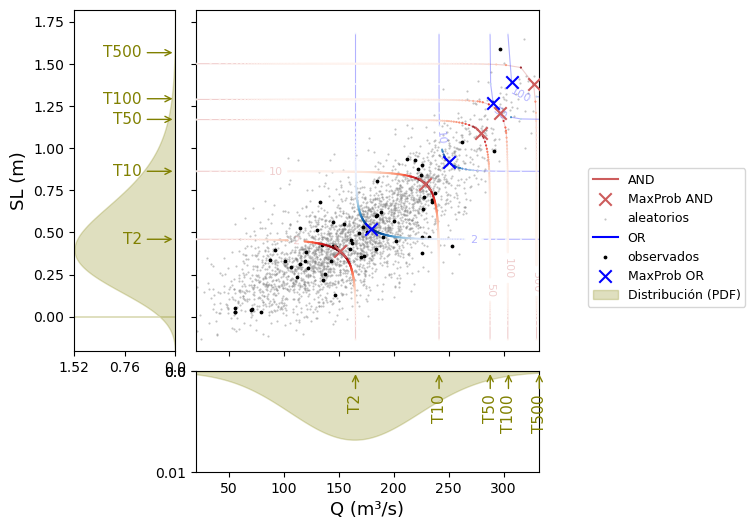
\includegraphics[width=\linewidth]{figures/fig_copula_joint_ret}
  \caption{Diagrama de períodos de retorno conjuntos AND y OR para un dataset sintético de caudal máximo ($Q_{\max}$, m$^3$/s) y nivel del mar (m) con cópula de Gumbel ajustada ($\tau_K \approx 0{,}52$). Las isolíneas AND (rojo) representan la condición de excedencia simultánea de ambas variables; las isolíneas OR (azul) la excedencia de al menos una de ellas. Los marcadores $\times$ señalan el \textsc{mpde} para cada período de retorno. Las distribuciones marginales ajustadas se muestran en los ejes superior y derecho. Elaboración propia a partir del notebook \texttt{compound\_flooding.ipynb}.}
  \label{fig:copula_joint_ret}
\end{figure}

\begin{figure}[htbp]
  \centering
  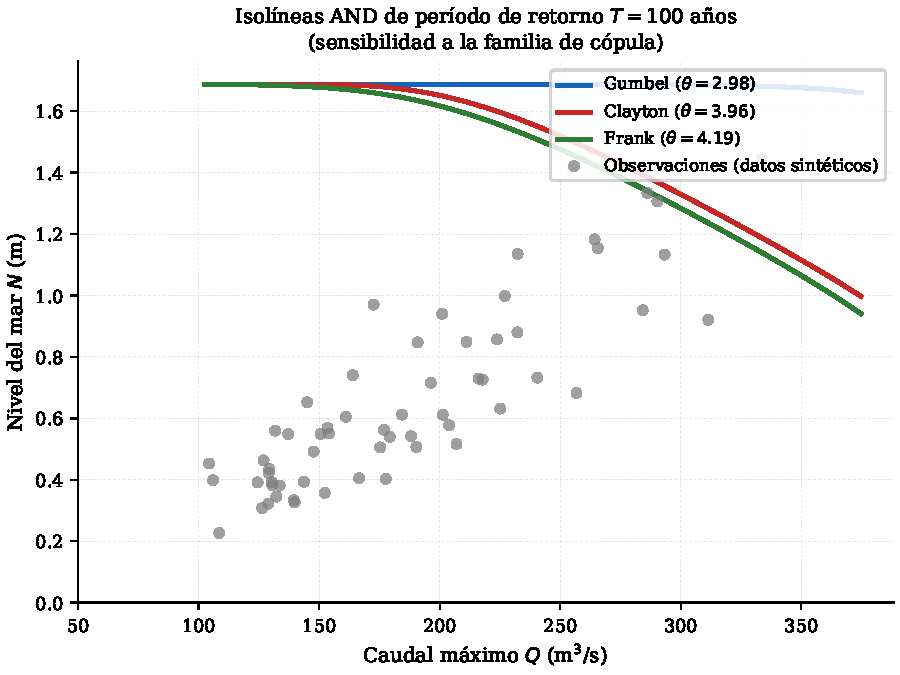
\includegraphics[width=\linewidth]{figures/fig_copula_familias}
  \caption{Comparación de las isolíneas AND de período de retorno $T=100$ años para tres familias de cópulas (Gumbel, Clayton y Frank) ajustadas sobre el mismo dataset. La familia Gumbel concentra la probabilidad conjunta en la cola superior (dependencia extrema simultánea), Clayton en la cola inferior y Frank produce isolíneas simétricas. La elección de familia modifica significativamente la región de diseño para el mismo período de retorno. Elaboración propia a partir del notebook \texttt{compound\_flooding.ipynb}.}
  \label{fig:copula_familias}
\end{figure}

\subsection{Interpolación geoestadística}

El módulo de interpolación espacial, \path{spatial_analysis.interpolation}, proporciona las clases \texttt{IDWInterpolator} y \texttt{KrigingInterpolator} para interpolar campos de estaciones a malla regular, además de \texttt{GaussianProcessInterpolator} para regresión por proceso gaussiano con covariables. Soporta así dos familias de métodos: inverso de la distancia ponderado (IDW) y kriging ordinario o universal con deriva externa (elevación, coordenadas u otra covariable). El kriging universal con elevación como variable auxiliar fue el método utilizado en el caso de Mallorca \parencite{navas2019mallorca} para la asignación de precipitación a subcuencas desde los pluviómetros disponibles.

La interpolación se trata como un módulo de análisis espacial, no como un mero preprocesado gráfico. La elección entre IDW, kriging ordinario y kriging universal depende de la densidad de estaciones, la relación con covariables topográficas y la escala del fenómeno. Cuando se usa elevación o precipitación media satelital como deriva externa, el módulo conserva esa covariable junto al campo interpolado para que el resultado pueda reproducirse.

\subsection{Modelos jerárquicos bayesianos}

El módulo \path{spatial_analysis.bayes_hierarchical} implementa la clase \texttt{HierarchicalGEV} para análisis regional con estructura jerárquica. El modelo asume que los parámetros de la distribución de extremos en cada localización son realizaciones de una distribución común de nivel superior (hiperpriors poblacionales), lo que permite transferir información entre estaciones y estimar cuantiles en puntos con muestras cortas. La inferencia se realiza mediante MCMC completo, con PyMC como motor por defecto y PyStan \parencite{carpenter2017stan} como alternativa. La clase expone \texttt{.fit(data\_dict)} para calibrar el modelo, \texttt{.posterior\_summary()} para resumir la posterior de los parámetros poblacionales y por estación, y \texttt{.return\_levels(credible=0.95)} para los cuantiles de período de retorno con su intervalo de credibilidad. A diferencia de enfoques basados en aproximaciones de Laplace anidadas (INLA) \parencite{rue2009inla}, la implementación actual no aproxima la posterior: la calcula por muestreo completo, lo que es más costoso computacionalmente pero evita las hipótesis de regularidad que exige INLA.

\section{Generación estocástica}

\subsection{Precipitación estocástica: NEOPRENE y CoSMoS}

El submódulo \texttt{stochastic\_generation} integra NEOPRENE como librería backend para generación estocástica de precipitación \parencite{diezsierra2023neoprene}. La clase \texttt{NSRPModel} envuelve la implementación puntual del proceso de Neyman-Scott de pulsos rectangulares \parencite{rodriguezituribe1987,rodriguezituribe1988}. El proceso NSRP es un modelo de eventos clusterizados donde cada tormenta madre genera un número aleatorio de células de lluvia con inicio, intensidad y duración extraídas de distribuciones paramétricas. La calibración ajusta los parámetros del proceso para reproducir estadísticos observados de la serie horaria o diaria: media, varianza, probabilidad de precipitación nula, correlación lag-1 y coeficiente de variación. La clase \texttt{STNSRPModel} envuelve la implementación multisitio de NEOPRENE, que extiende NSRP a estaciones correlacionadas y permite la generación de campos de precipitación espacialmente coherentes.

La diferencia entre \texttt{NSRPModel} y \texttt{STNSRPModel} es operativa. El primero es adecuado cuando se necesita una serie sintética representativa de un punto o estación; el segundo se utiliza cuando la coherencia espacial entre estaciones es parte del problema, por ejemplo para alimentar subcuencas simultáneamente o reconstruir campos multisitio. En ambos casos, \pyhydra actúa como envoltorio de NEOPRENE y estandariza entradas, salidas y configuración, pero no modifica la formulación estadística del modelo.

La serie temporal de caudal se puede también generar estocásticamente mediante el conjunto de funciones que el submódulo \texttt{stochastic\_generation.point} expone como envoltorio de la librería externa CoSMoS (\emph{Complete Stochastic Modelling Solution}) \parencite{papalexiou2018storm}: \texttt{fit\_distribution} y \texttt{fit\_acs} calibran, respectivamente, la marginal y la estructura de autocorrelación estacional; \texttt{analyze\_ts} encadena ambos ajustes sobre una serie diaria; y \texttt{simulate\_ts}/\texttt{generate\_ts} producen las realizaciones sintéticas. Este enfoque genera series preservando simultáneamente la distribución marginal, la dependencia temporal y la estacionalidad de la variable simulada. En \pyhydra se utiliza como generador general de series hidrológicas cuando el objetivo es producir realizaciones temporales largas de caudal o precipitación a partir de una estructura estadística calibrada, en contraste con NEOPRENE, que contiene NSRP y STNSRP y representa explícitamente la estructura física de la precipitación mediante tormentas y células.

La elección entre NEOPRENE y CoSMoS depende del objeto del estudio. NEOPRENE es preferible cuando interesa representar precipitación como proceso de tormentas y células, especialmente en aplicaciones espaciales de lluvia. CoSMoS es más general cuando la variable puede tratarse como serie temporal con una marginal y una estructura de dependencia temporal objetivo, por ejemplo caudal o variables hidroclimáticas agregadas. Mantener ambos enfoques permite cubrir problemas de inundación por eventos y problemas de recurso hídrico o clima de largo plazo.

\subsection{Campos espaciales}

El módulo \texttt{stochastic\_generation.fields} genera campos de precipitación en malla a partir de campos analíticos parametrizados o por interpolación de realizaciones puntuales del STNSRP. Sus salidas son \texttt{DataArray} con dimensiones \texttt{(realización, tiempo, lat, lon)}, compatibles directamente con los módulos de downscaling híbrido y de modelización hidrológica.

Estos campos no sustituyen a un modelo atmosférico regional; son escenarios estadísticos espacialmente coherentes para alimentar modelos hidrológicos o explorar sensibilidad. Por ello, el módulo registra la semilla, la malla, los parámetros de variograma o interpolación y las estaciones de origen. Sin esos metadatos, un campo sintético sería difícilmente auditable.

\section{Corrección de sesgo}

El submódulo \texttt{climate.bias\_correction} proporciona cuatro variantes para corregir las diferencias sistemáticas entre modelos climáticos y observaciones de referencia \parencite{teutschbein2012biascorrection}, accesibles mediante la función \texttt{delta\_method} y la clase \texttt{BiasCorrection}:

\begin{description}
  \item[\texttt{delta\_method}] Corrección aditiva (para temperatura) o multiplicativa (para precipitación) que aplica el cambio relativo del modelo climático mes a mes entre el período histórico de control y el período futuro, preservando el valor medio observado. Es el método más conservador y el preferido cuando se quiere minimizar la interferencia sobre la señal de cambio climático.

  \item[\texttt{BiasCorrection.quantile\_mapping}] Mapeo cuantil empírico aditivo (EQM): mapea la distribución empírica del modelo en el período histórico sobre la distribución observada y aplica la corrección resultante al período de proyección.

  \item[\texttt{BiasCorrection.quantile\_deltamapping}] Variante multiplicativa del mapeo cuantil empírico (QDM), más adecuada para precipitación.

  \item[\texttt{BiasCorrection.scaled\_distribution\_mapping}] SDM paramétrico \parencite{switanek2017sdm}: ajusta distribuciones gamma (precipitación) o normal (temperatura) a las tres series y preserva explícitamente los cambios de frecuencia e intensidad proyectados por el modelo climático. Es la variante recomendada cuando la magnitud del cambio en extremos es relevante.
\end{description}

El método \texttt{BiasCorrection.fit\_transform(obs, hist, future, var, method=\text{\textquotesingle}delta\text{\textquotesingle})} ofrece un punto de entrada único a las cuatro variantes sin necesidad de instanciar la clase explícitamente.

Ambos métodos fueron aplicados en los estudios de los países andinos \parencite{paz2019idb,deljesus2020andinos} y en SIMPCCe \parencite{navas2025simpce}, con proyecciones CMIP5 y CMIP6 respectivamente.

En \pyhydra, la corrección de sesgo se implementa como transformación explícita entre una serie o campo del modelo climático y una referencia observacional. El módulo conserva el período de calibración, la fuente observada, el modelo, el escenario y la variante de corrección. Esta trazabilidad es crítica porque dos estudios con el mismo modelo CMIP6 pueden producir resultados distintos si cambian el período histórico, la fuente observacional o la variante de mapeo cuantil.

\section{Downscaling híbrido}

El submódulo \texttt{climate.hybrid\_downscaling} implementa la cadena metodológica que conecta eventos sintéticos o escenarios seleccionados con mapas de inundación a escala de cuadrícula \parencite{navas2019mallorca,navas2024calle30}. La cadena consta de cuatro pasos:

\begin{enumerate}
  \item \textbf{Selección de eventos representativos (MaxDiss).} La función \path{maxdiss}, situada en \path{hybrid_downscaling.reconstruction}, selecciona un subconjunto de $n$ escenarios representativos del espacio total de eventos mediante el algoritmo de máxima disimilitud \parencite{camus2011maxdiss}. El algoritmo construye iterativamente un conjunto que maximiza la distancia mínima entre cualquier par de escenarios, cubriendo el espacio de variabilidad con el mínimo número de simulaciones. El submódulo \path{hybrid_downscaling.classification} complementa esta selección con \texttt{HydrographClassifier}, que agrupa formas de hidrograma por PCA y \emph{k}-means para organizar espacialmente los tipos representativos.

  \item \textbf{Simulación hidráulica del subconjunto.} Los $n$ eventos seleccionados se simulan con el modelo hidráulico (HEC-RAS, SFINCS) para obtener mapas de calado y velocidad.

  \item \textbf{Reconstrucción por vecinos próximos (k-NN).}\par
  La clase \path{FloodMapInterpolator} forma parte del submódulo de interpolación del downscaling híbrido. Entrena un modelo k-NN sobre los descriptores de evento y los mapas simulados. Una vez entrenado, reconstruye el mapa de inundación de cualquier evento del conjunto completo a partir de la interpolación ponderada de sus $k$ vecinos más próximos en el espacio de descriptores. En el caso de Calle 30 \parencite{navas2024calle30}, este enfoque permitió reconstruir miles de escenarios de inundación a partir de un conjunto de simulaciones explícitas mucho menor.

  \item \textbf{Mapas de período de retorno.} La función \texttt{pixel\_return\_period} en \texttt{hybrid\_downscaling.return\_period} calcula, para cada pixel de la malla, la distribución de calado máximo sobre el conjunto de escenarios y sus tasas de ocurrencia anuales, produciendo un mapa de nivel de retorno para cada período de retorno solicitado. La función \texttt{save\_return\_period\_geotiffs} exporta estos mapas en formato GeoTIFF georreferenciado.
\end{enumerate}

La \cref{fig:maxdiss_downscaling} resume la lógica operativa del método. El bloque superior representa la cadena estadística: datos históricos, extracción y descripción de eventos, generación sintética de $N$ realizaciones y selección MaxDiss del subconjunto representativo $n$. El bloque inferior representa la cadena física: preparación del dominio hidráulico, simulación explícita de los $n$ eventos seleccionados, construcción de una biblioteca de mapas de calado y reconstrucción k-NN de los mapas del conjunto completo. Las salidas de auditoría intermedias (tabla de eventos, listado de casos a simular, GeoTIFF intermedios) garantizan la trazabilidad de cada resultado.

\begin{figure}[!htbp]
\centering
\resizebox{\textwidth}{!}{%
\begin{tikzpicture}[
  font=\scriptsize,
  node distance=0.78cm and 0.78cm,
  arr/.style={-Stealth, line width=0.8pt, color=tg55},
  data/.style={rectangle, rounded corners=3pt, draw=blue!55!black, fill=blue!8,
	               text width=2.48cm, minimum height=0.78cm, align=center},
  stat/.style={rectangle, rounded corners=3pt, draw=orange!70!black, fill=orange!12,
	               text width=2.48cm, minimum height=0.78cm, align=center},
  model/.style={rectangle, rounded corners=3pt, draw=teal!65!black, fill=teal!10,
	                text width=2.48cm, minimum height=0.78cm, align=center},
  outputbox/.style={rectangle, rounded corners=3pt, draw=red!55!black, fill=red!8,
	              text width=2.48cm, minimum height=0.78cm, align=center},
  group/.style={rectangle, rounded corners=5pt, draw=tg40, dashed, inner sep=0.18cm},
  dot/.style={circle, fill=#1, minimum size=0.16cm, inner sep=0}
]

% Main methodological chain
\node[data] (obs) {Datos históricos\\caudal o lluvia};
\node[stat, right=of obs] (events) {Extracción y\\descripción de eventos};
\node[stat, right=of events] (synthetic) {Generación sintética\\$N$ eventos};
\node[stat, right=of synthetic] (maxdiss) {MaxDiss\\$n \ll N$ eventos};

\node[model, below=1.05cm of maxdiss] (hydraulic) {Simulación hidráulica\\eventos $n$};
\node[model, left=of hydraulic] (maps) {Biblioteca\\calado/velocidad};
\node[model, left=of maps] (knn) {Reconstrucción k-NN\\resto de eventos};
\node[outputbox, left=of knn] (risk) {Mapas finales\\período de retorno};

\draw[arr] (obs) -- (events);
\draw[arr] (events) -- (synthetic);
\draw[arr] (synthetic) -- (maxdiss);
\draw[arr] (maxdiss.south) -- (hydraulic.north);
\draw[arr] (hydraulic) -- (maps);
\draw[arr] (maps) -- (knn);
\draw[arr] (knn) -- (risk);

% Inputs from hydraulic domain
\node[data, below=0.85cm of hydraulic] (terrain) {MDE, rugosidad,\\malla y contornos};
\draw[arr] (terrain.north) -- (hydraulic.south);

% Audit products
\node[outputbox, above=0.75cm of events] (audit1) {Tabla de eventos\\y descriptores};
\node[outputbox, above=0.75cm of maxdiss] (audit2) {Listado de casos\\a simular};
\node[outputbox, below=0.75cm of maps] (audit3) {GeoTIFF/NetCDF\\intermedios};
\draw[arr] (events.north) -- (audit1.south);
\draw[arr] (maxdiss.north) -- (audit2.south);
\draw[arr] (maps.south) -- (audit3.north);

\end{tikzpicture}
}
\caption{Esquema operativo del downscaling híbrido implementado en \hydra. La metodología separa la generación estadística masiva de eventos ($N$ escenarios) de la simulación hidráulica completa: MaxDiss selecciona un subconjunto representativo $n \ll N$ que cubre el espacio de variabilidad, ese subconjunto se simula con el modelo físico, y los mapas del conjunto restante se reconstruyen por k-NN. Las salidas de auditoría intermedias permiten trazar cada resultado hasta su configuración de datos y simulación. Elaboración propia.}
\label{fig:maxdiss_downscaling}
\end{figure}

Este flujo, denominado \emph{downscaling híbrido} porque combina selección estadística con reconstrucción por aprendizaje automático, reduce el coste computacional de la metodología estocástica en varios órdenes de magnitud respecto a simular todos los eventos \parencite{deljesus2024downscaling}. Su validez exige descriptores hidráulicamente informativos y un subconjunto MaxDiss representativo del espacio de variabilidad.

\subsection{Validación de la reconstrucción k-NN}
\label{sec:validacion_knn}

La reconstrucción k-NN es la pieza que hace viable la metodología estocástica, y por tanto su error debe cuantificarse en cada aplicación en lugar de asumirse. El protocolo de validación integrado en el flujo es la validación cruzada sobre el propio subconjunto simulado: se excluye una simulación (o un pliegue de ellas), se reconstruye su mapa a partir de las restantes mediante \texttt{FloodMapInterpolator} y se compara la reconstrucción con la simulación física excluida. Sobre cada par reconstruido--simulado se calculan tres familias de métricas complementarias: error de calado por píxel (RMSE y sesgo medio, restringidos a la zona inundada); acierto en extensión sobre un umbral de calado, resumido mediante el índice de acierto crítico (CSI) y las tasas de sobrepredicción e infrapredicción; y error en los cuantiles altos de la distribución de calados, que son los que gobiernan los mapas de período de retorno.

Este análisis cumple tres funciones operativas. Primero, dimensionar el subconjunto MaxDiss: si el error de validación cruzada no se estabiliza al aumentar $n$, el subconjunto no cubre suficientemente el espacio de variabilidad. Segundo, diagnosticar los descriptores: errores concentrados en un tipo de evento indican que el espacio de características no captura alguna dimensión hidráulicamente relevante (forma del hidrograma, simultaneidad entre subcuencas). Tercero, acotar la incertidumbre de reconstrucción que se propaga a los mapas de período de retorno, de modo que pueda declararse junto al resto de fuentes de incertidumbre del estudio. En las aplicaciones de la línea (Mallorca, Calle 30, Panamá) la verificación se realizó mediante la comparación de mapas reconstruidos frente a simulados durante el desarrollo de cada estudio; la sistematización de estas métricas como salida estándar del módulo, con informe automático de validación cruzada por caso, forma parte de los criterios de aceptación recogidos en el \cref{ch:casos_estudio}.
